 %% ==========================================================================
%% Elsevier Journal Paper — elsarticle class (Two-Column Layout)
%% Title: An Ultra-Low-Power 10-Transistor 1-Bit Magnitude Comparator
%%        Using Gate Diffusion Input Technique
%% ==========================================================================

\documentclass[final,5p,times,twocolumn]{elsarticle}

%% ---------- PACKAGES ----------
\usepackage[T1]{fontenc}
\usepackage[utf8]{inputenc}
\usepackage{amsmath,amssymb}
\usepackage{graphicx}
\usepackage{float}
\usepackage{booktabs}
\usepackage{multirow}
\usepackage{array}
\usepackage{tabularx}
\usepackage{url}
\usepackage{xcolor}
\usepackage{colortbl}

%% ---------- MICROSOFT WORD TABLE STYLING ----------
\definecolor{worddarkblue}{HTML}{2F5597}   % Word Accent 1 Dark Blue (Header)
\definecolor{wordlightblue}{HTML}{D9E1F2}  % Word Accent 1 Light Blue (Highlight / Totals)
\definecolor{wordzebra}{HTML}{F2F5F9}      % Word Soft Alternating Row Tint
\definecolor{wordborder}{HTML}{A6B9D0}     % Word Grid Line Soft Steel Blue
\usepackage[hidelinks]{hyperref}

%% Ensure justified alignment and avoid overfull margins in 2-column mode
\sloppy
\emergencystretch=1.5em

\graphicspath{{./}{../}}

%% ---------- JOURNAL NAME ----------
\journal{Microelectronics Journal}

%% ==========================================================================
\begin{document}

\begin{frontmatter}

%% ---------- TITLE ----------
\title{An Ultra-Low-Power 10-Transistor 1-Bit Magnitude Comparator Using Gate Diffusion Input Technique}

%% ---------- AUTHORS ----------
\author[iiuc]{Shahrear Hossain Shawon\corref{cor1}}
\ead{sshahrearhossain@gmail.com}

\author[iiuc]{Riazul Islam}
\ead{iriazul74@gmail.com}

\cortext[cor1]{Corresponding author.}

\affiliation[iiuc]{organization={Department of Electrical and Electronic Engineering, International Islamic University Chittagong},
            city={Chittagong},
            country={Bangladesh}}

%% ---------- ABSTRACT ----------
\begin{abstract}
Digital magnitude comparators serve as indispensable arithmetic building blocks in modern Very Large Scale Integration (VLSI) systems, including arithmetic logic units, flash analog-to-digital converters, and data sorting engines. Conventional static Complementary Metal-Oxide-Semiconductor (CMOS) implementations of 1-bit comparators typically require 32 transistors, resulting in elevated power dissipation and silicon area overhead. This paper presents the design, transistor-level implementation, and comprehensive performance evaluation of an ultra-low-power 1-bit magnitude comparator based on the Gate Diffusion Input (GDI) technique. The proposed architecture generates all three comparison outputs ($A>B$, $A=B$, and $A<B$) using only 10 transistors, achieving a 68.75\% reduction in device count over the standard static CMOS topology. The circuit was modeled and simulated using LTSpice with the 180\,nm Berkeley Predictive Technology Model at a supply voltage of 1.8\,V. Simulation results demonstrate an average power dissipation of 34.18\,pW, a propagation delay of 336\,ps for the equality output, and a Power-Delay Product (PDP) of $1.14\times 10^{-5}$\,fJ. Compared with the conventional static CMOS design, the proposed GDI comparator achieves a 73.83\% reduction in power consumption, a 15.59\% improvement in switching speed, and a 77.65\% improvement in energy efficiency. Benchmarking against four published comparator architectures confirms that the proposed design attains the lowest PDP among all evaluated topologies. Multi-node scaling evaluations across 180\,nm, 90\,nm, and 45\,nm technology regimes further validate consistent performance scalability. The proposed GDI comparator is well-suited for deployment in battery-operated, energy-harvesting, and biomedical VLSI applications.
\end{abstract}

%% ---------- KEYWORDS ----------
\begin{keyword}
Gate Diffusion Input (GDI) \sep magnitude comparator \sep low-power VLSI \sep CMOS logic design \sep Power-Delay Product \sep Predictive Technology Model
\end{keyword}

\end{frontmatter}

%% ==========================================================================
%% 1. INTRODUCTION
%% ==========================================================================
\section{Introduction}
\label{sec:introduction}

The relentless scaling of semiconductor technology over the past several decades has enabled the integration of billions of transistors onto a single silicon die, powering a diverse range of computing platforms from high-performance server processors to ultra-compact wearable health monitors \cite{rabaey2003}. As transistor gate lengths shrink below the 100\,nm threshold, the interplay between dynamic switching power and static leakage current has fundamentally altered the power dissipation landscape of digital integrated circuits \cite{roy2003,narendra2006}. In battery-operated portable electronics, wireless sensor nodes, and implantable biomedical devices, power consumption has emerged as the single most critical design constraint, often surpassing speed and area in overall importance.

Among the foundational arithmetic building blocks of digital computing architectures, digital magnitude comparators occupy a particularly important position. These circuits accept two binary operands and generate outputs that indicate whether one operand is greater than, equal to, or less than the other. Comparator circuits find extensive deployment in arithmetic logic units (ALUs), central processing units (CPUs), digital signal processors (DSPs), data sorting networks, priority encoders, and high-speed flash analog-to-digital converters (ADCs) \cite{weste2011,kang2003}. The performance characteristics of comparator modules---namely propagation delay, power dissipation, and silicon area---directly influence the throughput, energy budget, and physical footprint of the larger digital systems in which they are embedded.

The conventional approach to implementing a 1-bit magnitude comparator employs static CMOS logic, which provides robust noise margins, full rail-to-rail output voltage swing, and predictable switching behavior. However, a standard static CMOS realization of a complete 1-bit comparator typically demands 32 transistors, resulting in substantial parasitic capacitance, elevated dynamic and leakage power consumption, and a relatively large silicon die area \cite{baker2010}. Several alternative logic families have been explored to reduce these overheads, including Pass Transistor Logic (PTL) and Transmission Gate Logic (TGL). While PTL can reduce transistor count, it suffers from threshold voltage drops that degrade output voltage levels and noise margins. TGL provides full-swing outputs through complementary NMOS--PMOS switch pairs but requires additional inverters, increasing the overall device count \cite{rabaey2003}.

The Gate Diffusion Input (GDI) technique, introduced by Morgenshtein et al. \cite{morgenshtein2002}, offers an elegant circuit design paradigm that permits the realization of complex Boolean logic functions using a significantly reduced number of transistors compared to conventional CMOS and pass-transistor implementations. A basic GDI cell comprises only two transistors---one PMOS and one NMOS---sharing a common gate terminal and a common drain (output) terminal. Unlike standard CMOS inverter topologies, where the PMOS source is tied to $V_{DD}$ and the NMOS source is tied to ground, the GDI cell routes arbitrary input signals to the diffusion (source) terminals, enabling the synthesis of diverse logic functions such as AND, OR, MUX, and XOR with minimal device overhead \cite{morgenshtein2002,morgenshtein2014}.

Recent investigations into comparator circuit design have explored various strategies for improving power and delay performance. Sharma et al. \cite{sharma2025} presented a hybrid PTL--GDI--TGL comparator with an impressively low 5.5\,ps delay, but the design requires 24 transistors and consumes 7.3\,$\mu$W of average power. Lubaba et al. \cite{lubaba2020} designed a 2-bit hybrid comparator using Pass Transistor, Transmission Gate, and conventional CMOS logic in 90\,nm technology, achieving 192\,ps delay but with microwatt-level power dissipation (7.792\,$\mu$W). Tailor et al. \cite{tailor2019} employed Multi-Threshold CMOS (MTCMOS) with forced stack techniques, reporting a delay of 330.61\,ps and power consumption of 48.12\,pW; however, the dual-threshold fabrication process introduces additional manufacturing complexity and cost. Kumar and Kumar \cite{kumar2017} applied transistor stacking techniques to a static CMOS comparator in 180\,nm technology, achieving reduced leakage power but with a 45+ transistor count and a propagation delay of 49.38\,ns. These existing works highlight a persistent trade-off: designs that achieve aggressive delay targets tend to exhibit high active power consumption, while ultra-low-power topologies often sacrifice switching speed or require specialized fabrication processes.

This paper addresses these limitations by presenting a pure GDI-based 1-bit magnitude comparator that achieves picowatt-level power consumption with sub-nanosecond switching delay using only 10 transistors. The principal contributions of this work are as follows:

\begin{enumerate}
    \item A complete 10-transistor GDI-based 1-bit magnitude comparator generating all three comparison outputs ($A>B$, $A=B$, $A<B$) with minimal device count and no requirement for specialized fabrication processes.
    \item A systematic four-way performance benchmarking against static CMOS (32T), Pass Transistor Logic (10T), and Transmission Gate Logic (16T) comparators under identical 180\,nm PTM simulation conditions.
    \item A comprehensive comparative analysis against four published comparator architectures from the literature, demonstrating that the proposed design achieves the lowest Power-Delay Product among all evaluated topologies.
    \item A multi-node technology scaling evaluation across 180\,nm, 90\,nm, and 45\,nm Predictive Technology Model decks, confirming sustained performance scalability.
\end{enumerate}

The remainder of this paper is organized as follows. Section~\ref{sec:gdi_background} reviews the GDI cell structure and its fundamental logic functions. Section~\ref{sec:proposed_design} describes the proposed comparator architecture and its Boolean-to-GDI mapping. Section~\ref{sec:methodology} details the simulation methodology and testbench configuration. Section~\ref{sec:results} presents the simulation results and performance comparisons. Section~\ref{sec:discussion} provides detailed analysis and discussion. Section~\ref{sec:conclusion} draws conclusions and outlines directions for future research.


%% ==========================================================================
%% 2. GDI TECHNIQUE BACKGROUND
%% ==========================================================================
\section{Gate Diffusion Input technique: cell structure and logic functions}
\label{sec:gdi_background}

The Gate Diffusion Input methodology was first proposed by Morgenshtein, Fish, and Wagner as an alternative to conventional CMOS logic for low-power digital circuit design \cite{morgenshtein2002}. The fundamental GDI cell, depicted in Fig.~\ref{fig:gdi_cell}, consists of two complementary transistors arranged in a topology that closely resembles a standard CMOS inverter. The PMOS transistor (M1) and the NMOS transistor (M2) share a common gate terminal, designated as input $G$, and a common drain connection that forms the cell output. The distinguishing characteristic of the GDI structure lies in its diffusion terminal assignments: the source of the PMOS transistor is driven by an independent input signal $P$, while the source of the NMOS transistor receives a separate input signal $N$. This three-input configuration ($G$, $P$, $N$) enables a single GDI cell to implement multiple logic functions by simply altering the signal assignments at its terminals, as summarized in Table~\ref{tab:gdi_functions}.

\begin{figure}[t]
    \centering
    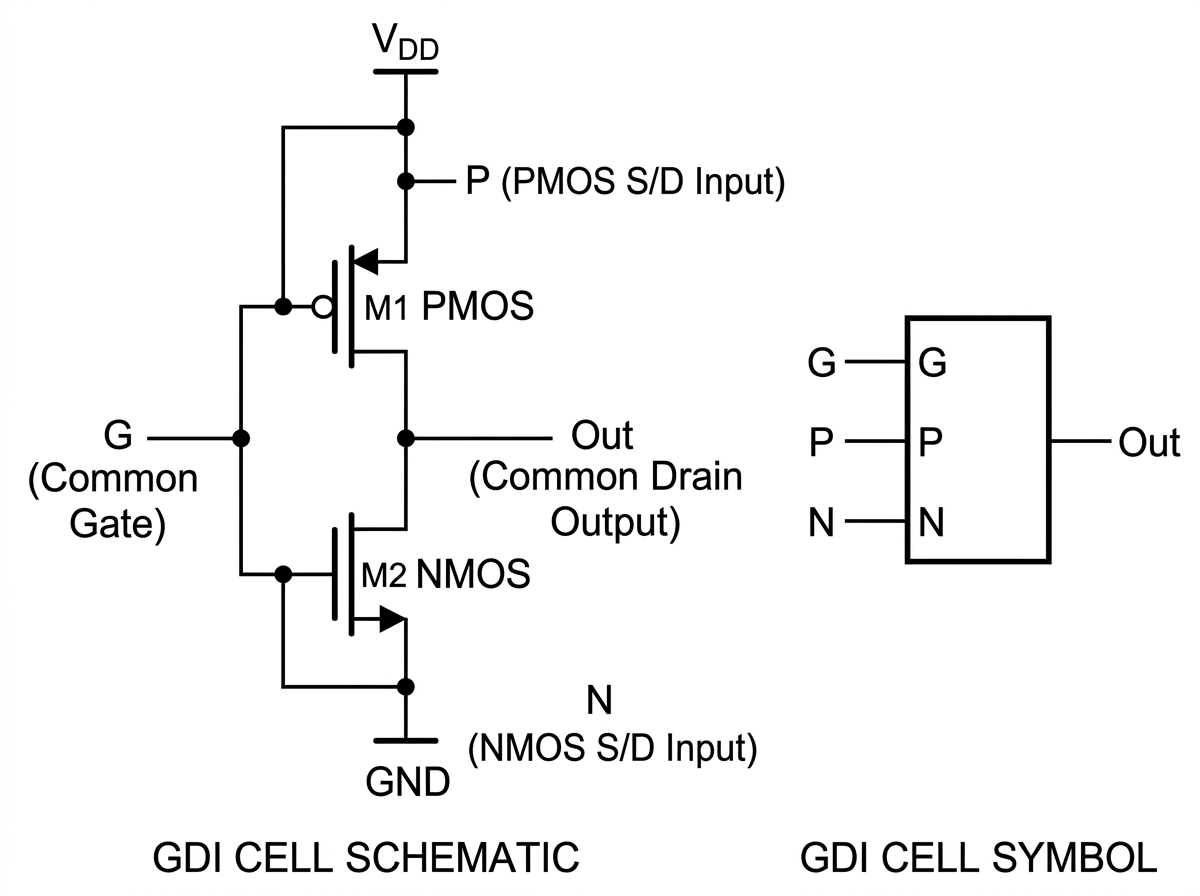
\includegraphics[width=0.88\columnwidth]{paper_gdi_cell_structure.jpg}
    \caption{Basic GDI cell: transistor-level schematic (left) and symbolic representation (right). The cell comprises one PMOS (M1) and one NMOS (M2) with a common gate ($G$) and common drain output. The PMOS source ($P$) and NMOS source ($N$) accept independent input signals.}
    \label{fig:gdi_cell}
\end{figure}

\begin{table}[t]
    \centering
    \caption{Logic functions realizable with a single GDI cell.}
    \label{tab:gdi_functions}
    \renewcommand{\arraystretch}{1.35}
    \setlength{\tabcolsep}{4pt}
    {\small
    \arrayrulecolor{wordborder}
    \begin{tabular}{|c|c|c|c|p{2.65cm}|}
        \hline
        \rowcolor{worddarkblue}
        \textcolor{white}{\textbf{Function}} & \textcolor{white}{\textbf{Output Expression}} & \textcolor{white}{\textbf{$N$}} & \textcolor{white}{\textbf{$P$}} & \textcolor{white}{\textbf{Description}} \\
        \hline
        F1  & $\bar{G} \cdot P$         & 0         & $B$       & AND with inverted gate \\
        \hline
        \rowcolor{wordzebra}
        F2  & $G + P$                   & $B$       & 1         & OR function \\
        \hline
        INV & $\bar{G}$                 & 0         & 1         & Standard inverter \\
        \hline
        \rowcolor{wordzebra}
        MUX & $\bar{G} P + G N$         & $B$       & $C$       & 2-to-1 multiplexer \\
        \hline
        XOR & $\bar{G} B + G \bar{B}$   & $\bar{B}$ & $B$       & Exclusive-OR \\
        \hline
        \rowcolor{wordzebra}
        XNOR & $\bar{G}\bar{B} + G B$   & $B$       & $\bar{B}$ & Exclusive-NOR \\
        \hline
    \end{tabular}
    }
\end{table}

The GDI technique offers several inherent advantages over conventional CMOS logic for low-power applications. First, since a single GDI cell can realize functions that would otherwise require four to twelve transistors in standard CMOS, the overall transistor count is substantially reduced. This reduction directly lowers parasitic gate, drain, and interconnect capacitances, which in turn decreases dynamic switching power ($P_{\text{dyn}} \propto C_{\text{load}} V_{DD}^{2} f$) and silicon die area. Second, fewer internal switching nodes translate into reduced short-circuit current during logic transitions, further lowering active power consumption. Third, the GDI cell provides direct signal routing through transistor diffusion terminals, eliminating the need for separate buffering stages and reducing propagation delay through critical signal paths \cite{morgenshtein2002,morgenshtein2014}.

A practical consideration for GDI circuits in bulk CMOS processes is the body effect. In standard bulk CMOS fabrication, NMOS body terminals are connected to ground and PMOS body terminals are tied to $V_{DD}$. When GDI input signals drive the source terminals to potentials other than these fixed references, the resulting source-body voltage ($V_{SB} \neq 0$) can shift the effective threshold voltage and slightly affect output voltage swing under certain load conditions. Nevertheless, for the logic functions employed in this work, simulations confirm that the output voltage degradation remains within acceptable noise margin bounds at the 180\,nm technology node with a 1.8\,V supply.


%% ==========================================================================
%% 3. PROPOSED GDI COMPARATOR DESIGN
%% ==========================================================================
\section{Proposed GDI-based 1-bit magnitude comparator}
\label{sec:proposed_design}

\subsection{Truth table and Boolean derivation}

A 1-bit magnitude comparator accepts two single-bit binary inputs, $A$ and $B$, and produces three mutually exclusive output signals: $A>B$ (greater-than), $A=B$ (equality), and $A<B$ (less-than). The truth table governing the operation of the comparator is presented in Table~\ref{tab:truth_table}.

\begin{table}[t]
    \centering
    \caption{Truth table for a 1-bit magnitude comparator.}
    \label{tab:truth_table}
    \renewcommand{\arraystretch}{1.35}
    \setlength{\tabcolsep}{12pt}
    {\small
    \arrayrulecolor{wordborder}
    \begin{tabular}{|c|c|c|c|c|}
        \hline
        \rowcolor{worddarkblue}
        \textcolor{white}{\textbf{Input $A$}} & \textcolor{white}{\textbf{Input $B$}} & \textcolor{white}{\textbf{$A>B$}} & \textcolor{white}{\textbf{$A=B$}} & \textcolor{white}{\textbf{$A<B$}} \\
        \hline
        0 & 0 & 0 & 1 & 0 \\
        \hline
        \rowcolor{wordzebra}
        0 & 1 & 0 & 0 & 1 \\
        \hline
        1 & 0 & 1 & 0 & 0 \\
        \hline
        \rowcolor{wordzebra}
        1 & 1 & 0 & 1 & 0 \\
        \hline
    \end{tabular}
    }
\end{table}

Applying Karnaugh-map minimization to the truth table entries yields the following simplified Boolean expressions for each output:

\begin{align}
    (A > B) &= A \cdot \overline{B} \label{eq:agb} \\
    (A = B) &= A \odot B = \overline{A \oplus B} = A B + \overline{A}\,\overline{B} \label{eq:aeb} \\
    (A < B) &= \overline{A} \cdot B \label{eq:alb}
\end{align}

These expressions reveal that the greater-than and less-than outputs are simple two-variable AND operations with one inverted input, while the equality output is an XNOR (equivalence) function. Each of these operations maps directly to a basic GDI cell configuration.

\subsection{Mapping Boolean functions to GDI cells}

The proposed design maps each comparator output to a dedicated 2-transistor GDI cell, as detailed below and summarized in Table~\ref{tab:gdi_mapping}.

\textbf{Greater-than output} ($A > B = A \cdot \overline{B}$): This function is implemented using a GDI cell configured as the F1 function. The gate terminal ($G$) is connected to input $B$, the PMOS source ($P$) is connected to input $A$, and the NMOS source ($N$) is tied to ground. When $B = 0$, the PMOS transistor conducts, passing the value of $A$ to the output. When $B = 1$, the NMOS transistor conducts, discharging the output to ground. The resulting output evaluates to $A \cdot \overline{B}$, requiring only 2 transistors.

\textbf{Less-than output} ($A < B = \overline{A} \cdot B$): This function employs a complementary GDI F1 configuration. The gate input ($G$) is connected to $A$, the PMOS source ($P$) is connected to $B$, and the NMOS source ($N$) is connected to ground. When $A = 0$, the PMOS passes $B$ to the output; when $A = 1$, the NMOS discharges the output. The output realizes $\overline{A} \cdot B$ with 2 transistors.

\textbf{Equality output} ($A = B = A \odot B$): The XNOR function is synthesized using a GDI multiplexer configuration. The gate input ($G$) is connected to $A$, the PMOS source ($P$) is connected to the inverted input $\overline{B}$, and the NMOS source ($N$) is connected to $B$. When $A = 0$, the PMOS conducts and passes $\overline{B}$; when $A = 1$, the NMOS conducts and passes $B$. The resulting output correctly implements the XNOR equivalence operation using 2 transistors.

\textbf{Input inversion stages}: Two standard 2-transistor CMOS inverters generate the complementary signals $\overline{A}$ and $\overline{B}$ required by the less-than output cell and the equality XNOR cell, respectively.

\begin{table}[t]
    \centering
    \caption{GDI cell terminal assignments for each comparator output.}
    \label{tab:gdi_mapping}
    \renewcommand{\arraystretch}{1.35}
    \setlength{\tabcolsep}{3.5pt}
    {\small
    \arrayrulecolor{wordborder}
    \begin{tabular}{|c|c|c|c|c|c|}
        \hline
        \rowcolor{worddarkblue}
        \textcolor{white}{\textbf{Output}} & \textcolor{white}{\textbf{Boolean Function}} & \textcolor{white}{\textbf{$G$}} & \textcolor{white}{\textbf{$P$}} & \textcolor{white}{\textbf{$N$}} & \textcolor{white}{\textbf{Transistors}} \\
        \hline
        $A > B$ & $A \cdot \overline{B}$ & $B$ & $A$ & GND & 2 \\
        \hline
        \rowcolor{wordzebra}
        $A < B$ & $\overline{A} \cdot B$ & $A$ & $B$ & GND & 2 \\
        \hline
        $A = B$ & $A \odot B$ (XNOR) & $A$ & $\overline{B}$ & $B$ & 2 \\
        \hline
        \rowcolor{wordzebra}
        Inverter $\overline{A}$ & $\overline{A}$ & $A$ & $V_{DD}$ & GND & 2 \\
        \hline
        Inverter $\overline{B}$ & $\overline{B}$ & $B$ & $V_{DD}$ & GND & 2 \\
        \hline
        \rowcolor{wordlightblue}
        \multicolumn{5}{|r|}{\textbf{Total transistor count:}} & \textbf{10} \\
        \hline
    \end{tabular}
    }
\end{table}

Combining the three output cells and two input inverters yields a complete 1-bit magnitude comparator implemented with a total of \textbf{10 transistors} (5 PMOS and 5 NMOS). This represents a 68.75\% reduction in transistor count compared to the conventional 32-transistor static CMOS design.

\subsection{Circuit schematic}

Fig.~\ref{fig:proposed_circuit} presents the transistor-level schematic of the proposed 10-transistor GDI comparator as captured in the LTSpice simulation environment. The circuit comprises two inverters ($M_{11}$, $M_{12}$ for $\overline{A}$ and $M_3$, $M_4$ for $\overline{B}$), an $A>B$ GDI cell ($M_9$, $M_{10}$), an $A<B$ GDI cell ($M_7$, $M_8$), and an $A=B$ XNOR GDI cell ($M_1$, $M_2$).

\begin{figure*}[t]
    \centering
    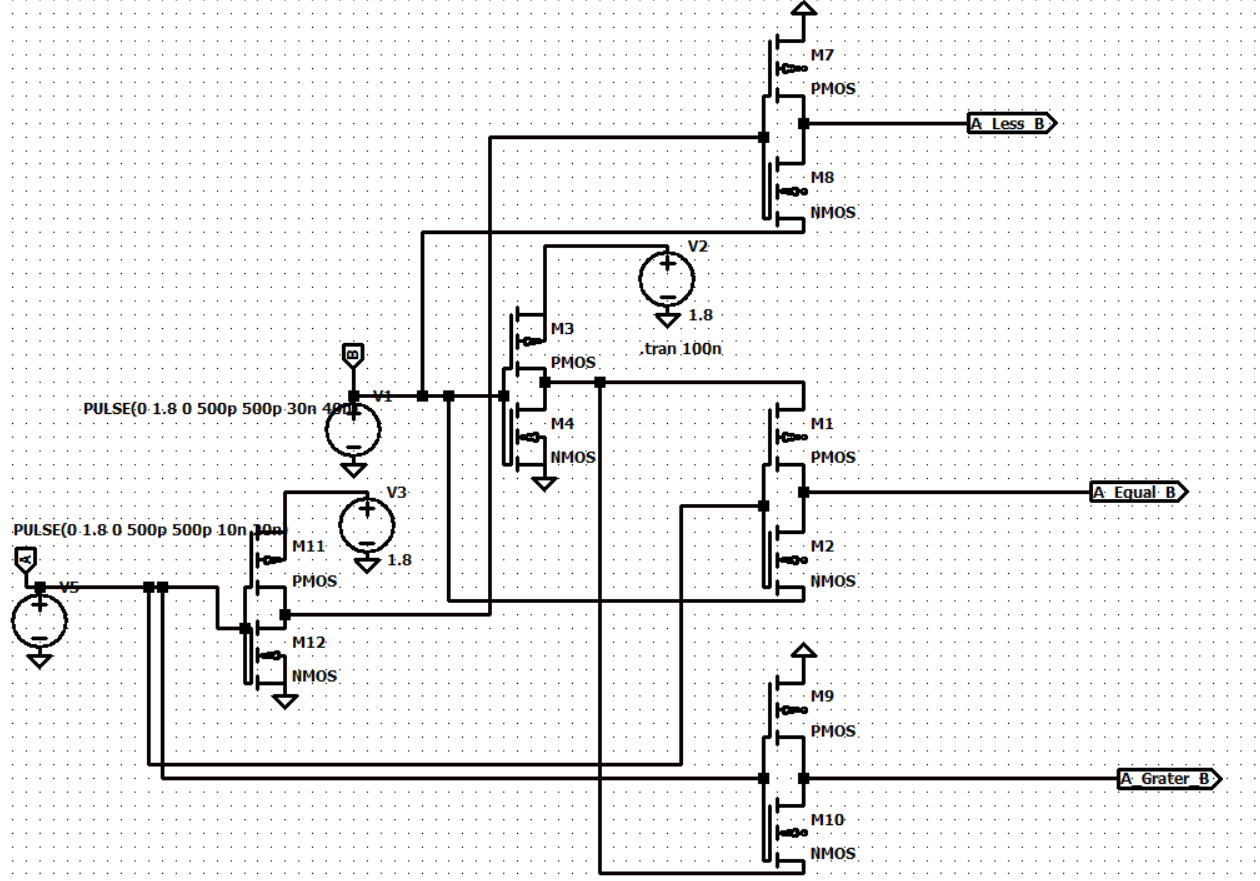
\includegraphics[width=0.88\textwidth]{Paper_my_Propose_GDI_Comparator.png}
    \caption{Transistor-level schematic of the proposed 10-transistor GDI-based 1-bit magnitude comparator implemented in LTSpice. The circuit generates all three outputs ($A>B$, $A=B$, $A<B$) using five GDI/inverter cells.}
    \label{fig:proposed_circuit}
\end{figure*}


%% ==========================================================================
%% 4. SIMULATION METHODOLOGY
%% ==========================================================================
\section{Simulation methodology}
\label{sec:methodology}

\subsection{Technology model and simulation platform}

All circuits were modeled and simulated using LTSpice XVII with the Berkeley Predictive Technology Model (PTM) at the 180\,nm bulk CMOS node \cite{zhao2007}. The PTM provides peer-reviewed BSIM3v3 Level 49 model parameters that are widely adopted in academic VLSI research for consistent and reproducible performance evaluation. Key model parameters include a gate oxide thickness of $t_{ox} = 4.0$\,nm, nominal NMOS threshold voltage $V_{th0,n} \approx 0.40$\,V, and nominal PMOS threshold voltage $V_{th0,p} \approx -0.42$\,V. The simulations were conducted at a nominal operating temperature of 27$^{\circ}$C under a supply voltage of $V_{DD} = 1.8$\,V.

\subsection{Transistor sizing}

To achieve reasonably balanced pull-up and pull-down drive capabilities, PMOS transistors were sized wider than NMOS transistors to compensate for the lower hole mobility ($\mu_p \approx 200$\,cm$^2$/V$\cdot$s) relative to electron mobility ($\mu_n \approx 500$\,cm$^2$/V$\cdot$s). The sizing ratio was chosen as $W_p / W_n = 2.0$. The channel dimensions for the 180\,nm node were: NMOS $W_n = 360$\,nm, $L_n = 180$\,nm ($W/L = 2$); PMOS $W_p = 720$\,nm, $L_p = 180$\,nm ($W/L = 4$). Proportionally scaled dimensions were used for the 90\,nm and 45\,nm evaluations.

\subsection{Benchmark comparator implementations}

To establish a rigorous comparative framework, three alternative 1-bit magnitude comparator topologies were implemented and simulated under identical technology models, supply voltages, and test conditions:

\textbf{Conventional Static CMOS}: Implemented using standard pull-up PMOS and pull-down NMOS networks realizing the complementary Boolean equations. The static CMOS design requires a total of \textbf{32 transistors} (16 PMOS, 16 NMOS) and serves as the primary reference baseline \cite{weste2011}.

\textbf{Transmission Gate Logic (TGL)}: Implemented using complementary NMOS--PMOS transmission switches. The TGL comparator uses \textbf{16 transistors} (8 PMOS, 8 NMOS), providing full-swing logic transmission at the cost of additional device overhead.

\textbf{Pass Transistor Logic (PTL)}: Implemented using single-channel NMOS pass transistors with complementary control signals. The PTL comparator requires \textbf{10 transistors} (5 PMOS, 5 NMOS), offering low device count but susceptibility to threshold voltage degradation ($V_{out} \approx V_{DD} - V_{th,n}$).

\subsection{Stimulus generation and testbench setup}

The simulation testbench was configured with two independent, synchronized pulse voltage sources driving inputs $A$ and $B$. To exhaustively exercise all four binary input combinations ($AB \in \{00, 01, 10, 11\}$), the input sources were parameterized as follows:
\begin{itemize}
    \item Input $A$: $V_{low} = 0$\,V, $V_{high} = 1.8$\,V, period $T_A = 40$\,ns, pulse width $PW_A = 20$\,ns, rise/fall times $t_r = t_f = 100$\,ps.
    \item Input $B$: $V_{low} = 0$\,V, $V_{high} = 1.8$\,V, period $T_B = 20$\,ns, pulse width $PW_B = 10$\,ns, rise/fall times $t_r = t_f = 100$\,ps.
\end{itemize}

Transient analysis was executed over a simulation interval of 80\,ns with a maximum time step of 10\,ps to ensure numerical accuracy.

\subsection{Performance metrics extraction}

Three key performance metrics were extracted from the simulation results:

\textbf{Propagation delay ($t_{pd}$)}: Measured between the 50\% voltage point of the triggering input transition and the 50\% voltage point of the corresponding output transition. Both low-to-high ($t_{pLH}$) and high-to-low ($t_{pHL}$) propagation delays were recorded, and the average propagation delay was computed as:
\begin{equation}
    t_{pd} = \frac{t_{pLH} + t_{pHL}}{2}
    \label{eq:tpd}
\end{equation}

\textbf{Average power dissipation ($P_{avg}$)}: Calculated by numerically integrating the instantaneous supply current $I(V_{DD})$ over the complete simulation interval $T_{sim} = 80$\,ns:
\begin{equation}
    P_{avg} = \frac{V_{DD}}{T_{sim}} \int_{0}^{T_{sim}} I_{DD}(t) \, dt
    \label{eq:pavg}
\end{equation}
This measurement captures both dynamic switching power and static leakage power.

\textbf{Power-Delay Product (PDP)}: Computed as the product of average power dissipation and propagation delay:
\begin{equation}
    \text{PDP} = P_{avg} \times t_{pd}
    \label{eq:pdp}
\end{equation}
The Power-Delay Product serves as the primary figure of merit for energy efficiency.


%% ==========================================================================
%% 5. RESULTS
%% ==========================================================================
\section{Results}
\label{sec:results}

\subsection{Functional verification}

Functional correctness was verified by applying synchronized pulse sequences to inputs $A$ and $B$, sweeping through all four binary input vectors. Table~\ref{tab:functional_ver} confirms that each comparator topology produces logically correct outputs for every input combination, with exactly one output asserted high at any given time.

\begin{table}[t]
    \centering
    \caption{Functional verification results across all comparator topologies.}
    \label{tab:functional_ver}
    \renewcommand{\arraystretch}{1.35}
    \setlength{\tabcolsep}{3.5pt}
    {\small
    \arrayrulecolor{wordborder}
    \begin{tabular}{|c|c|c|c|c|c|c|}
        \hline
        \rowcolor{worddarkblue}
        \textcolor{white}{\textbf{$A$}} & \textcolor{white}{\textbf{$B$}} & \textcolor{white}{\textbf{Expected}} & \textcolor{white}{\textbf{Static CMOS}} & \textcolor{white}{\textbf{TGL}} & \textcolor{white}{\textbf{PTL}} & \textcolor{white}{\textbf{GDI}} \\
        \hline
        0 & 0 & $A=B$ High & \checkmark & \checkmark & \checkmark & \checkmark \\
        \hline
        \rowcolor{wordzebra}
        0 & 1 & $A<B$ High & \checkmark & \checkmark & \checkmark & \checkmark \\
        \hline
        1 & 0 & $A>B$ High & \checkmark & \checkmark & \checkmark & \checkmark \\
        \hline
        \rowcolor{wordzebra}
        1 & 1 & $A=B$ High & \checkmark & \checkmark & \checkmark & \checkmark \\
        \hline
    \end{tabular}
    }
\end{table}

\subsection{Performance of the proposed GDI comparator}

Table~\ref{tab:gdi_performance} presents the measured timing, power, and energy parameters for each output of the proposed 10-transistor GDI comparator. The circuit exhibits balanced switching characteristics with propagation delays of 336\,ps ($A=B$), 345\,ps ($A>B$), and 353.50\,ps ($A<B$). The average power dissipation is 34.18\,pW, yielding a best-case PDP of $1.14 \times 10^{-5}$\,fJ.

\begin{table}[t]
    \centering
    \caption{Measured performance of proposed 10-transistor GDI comparator (180\,nm PTM, $V_{DD}$ = 1.8\,V).}
    \label{tab:gdi_performance}
    \renewcommand{\arraystretch}{1.35}
    \setlength{\tabcolsep}{3.5pt}
    {\small
    \arrayrulecolor{wordborder}
    \begin{tabular}{|l|c|c|c|}
        \hline
        \rowcolor{worddarkblue}
        \textcolor{white}{\textbf{Performance Metric}} & \textcolor{white}{\textbf{$A<B$}} & \textcolor{white}{\textbf{$A=B$}} & \textcolor{white}{\textbf{$A>B$}} \\
        \hline
        Transistor count & \multicolumn{3}{c|}{\textbf{10}} \\
        \hline
        \rowcolor{wordzebra}
        Rise time $t_r$ (10\%--90\%) & 553.03\,ps & 515.36\,ps & 532.37\,ps \\
        \hline
        Fall time $t_f$ (90\%--10\%) & 154.21\,ps & 157.73\,ps & 158.19\,ps \\
        \hline
        \rowcolor{wordzebra}
        Propagation delay $t_{pd}$ & 353.50\,ps & \textbf{336.00\,ps} & 345.00\,ps \\
        \hline
        Average power $P_{avg}$ & \multicolumn{3}{c|}{\textbf{34.18\,pW}} \\
        \hline
        \rowcolor{wordzebra}
        Power-Delay Product (PDP) & $1.20 \times 10^{-5}$\,fJ & $\mathbf{1.14 \times 10^{-5}}$\,\textbf{fJ} & $1.17 \times 10^{-5}$\,fJ \\
        \hline
    \end{tabular}
    }
\end{table}

The measured rise times (515--553\,ps) are consistently larger than fall times (154--158\,ps), reflecting the lower hole mobility in PMOS transistors responsible for pull-up transitions. The rise-to-fall time ratio of approximately 3.3:1 is consistent with the mobility ratio $\mu_n / \mu_p \approx 2.5$ and confirms that the chosen PMOS sizing ($W_p / W_n = 2$) provides reasonable switching characteristics.

\subsection{Benchmark comparator performance}

Table~\ref{tab:benchmark_results} presents the measured parameters for all three benchmark comparator topologies alongside the proposed GDI design. The static CMOS comparator dissipates 130.61\,pW with 32 transistors. The TGL comparator exhibits significantly higher average power (105.21\,$\mu$W) due to crowbar current flowing through the complementary transmission gate switches during signal transitions. The PTL design matches the 10-transistor count of the GDI circuit with 38.12\,pW power consumption but shows higher propagation delay (421.77\,ps) due to threshold voltage drop and body-effect degradation.

\begin{table*}[t]
    \centering
    \caption{Performance summary and comparative evaluation of benchmark comparator topologies (180\,nm PTM, 1.8\,V, $A=B$ output).}
    \label{tab:benchmark_results}
    \renewcommand{\arraystretch}{1.4}
    \setlength{\tabcolsep}{10pt}
    {\small
    \arrayrulecolor{wordborder}
    \begin{tabular}{|l|c|c|c|c|}
        \hline
        \rowcolor{worddarkblue}
        \textcolor{white}{\textbf{Metric}} & 
        \textcolor{white}{\textbf{Static CMOS}} & 
        \textcolor{white}{\textbf{TGL}} & 
        \textcolor{white}{\textbf{PTL}} & 
        \textcolor{white}{\textbf{Proposed GDI}} \\
        \hline
        Transistor count & 32 & 16 & 10 & \textbf{10} \\
        \hline
        \rowcolor{wordzebra}
        Device count reduction & Baseline & 50.00\% & 68.75\% & \textbf{68.75\%} \\
        \hline
        Average power $P_{avg}$ & 130.61\,pW & 105.21\,$\mu$W & 38.12\,pW & \textbf{34.18\,pW} \\
        \hline
        \rowcolor{wordzebra}
        Power savings vs.\ CMOS & Baseline & --- & 70.81\% & \textbf{73.83\%} \\
        \hline
        Delay $t_{pd}$ ($A=B$) & 398.09\,ps & 587.24\,ps & 421.77\,ps & \textbf{336.00\,ps} \\
        \hline
        \rowcolor{wordzebra}
        Speed improvement vs.\ CMOS & Baseline & $-47.51$\% & $-5.95$\% & \textbf{+15.59\%} \\
        \hline
        PDP ($A=B$) & $5.10 \times 10^{-5}$\,fJ & 61.78\,fJ & $1.60 \times 10^{-5}$\,fJ & $\mathbf{1.14 \times 10^{-5}}$\,\textbf{fJ} \\
        \hline
        \rowcolor{wordzebra}
        PDP improvement vs.\ CMOS & Baseline & --- & 68.63\% & \textbf{77.65\%} \\
        \hline
    \end{tabular}
    }
\end{table*}

\subsection{Comparative analysis with published literature}

Table~\ref{tab:literature_comparison} compares the proposed GDI comparator against four published comparator architectures, organized in reverse chronological order from 2025 to 2017. The proposed design achieves the lowest Power-Delay Product ($1.14 \times 10^{-5}$\,fJ) among all evaluated designs.

\begin{table*}[t]
    \centering
    \caption{Performance comparison with published comparator implementations arranged in reverse chronological order.}
    \label{tab:literature_comparison}
    \renewcommand{\arraystretch}{1.4}
    \setlength{\tabcolsep}{8pt}
    {\small
    \arrayrulecolor{wordborder}
    \begin{tabular}{|l|l|c|c|c|}
        \hline
        \rowcolor{worddarkblue}
        \textcolor{white}{\textbf{Reference}} & 
        \textcolor{white}{\textbf{Design Architecture}} & 
        \textcolor{white}{\textbf{Delay ($t_{pd}$)}} & 
        \textcolor{white}{\textbf{Power ($P_{avg}$)}} & 
        \textcolor{white}{\textbf{PDP (fJ)}} \\
        \hline
        Sharma et al. (2025) \cite{sharma2025} & PTL-GDI-TGL hybrid & 5.5\,ps & 7.3\,$\mu$W & 0.04 \\
        \hline
        \rowcolor{wordzebra}
        Lubaba et al. (2020) \cite{lubaba2020} & PTL-TG-CMOS hybrid (2-bit) & 0.192\,ns & 7.792\,$\mu$W & 1.496 \\
        \hline
        Tailor et al. (2019) \cite{tailor2019} & MTCMOS with forced stack & 330.61\,ps & 48.12\,pW & $1.59 \times 10^{-5}$ \\
        \hline
        \rowcolor{wordzebra}
        Kumar \& Kumar (2017) \cite{kumar2017} & CMOS with stacking & 49.38\,ns & 174.35\,pW & 0.0086 \\
        \hline
        \rowcolor{wordlightblue}
        \textbf{Proposed GDI (This work)} & \textbf{Pure GDI 10-transistor} & \textbf{336\,ps} & \textbf{34.18\,pW} & $\mathbf{1.14 \times 10^{-5}}$ \\
        \hline
    \end{tabular}
    }
\end{table*}

Fig.~\ref{fig:delay_comparison}, Fig.~\ref{fig:power_comparison}, and Fig.~\ref{fig:pdp_comparison} present bar chart visualizations of the propagation delay, average power dissipation, and Power-Delay Product comparisons across all evaluated designs, respectively.

\begin{figure}[t]
    \centering
    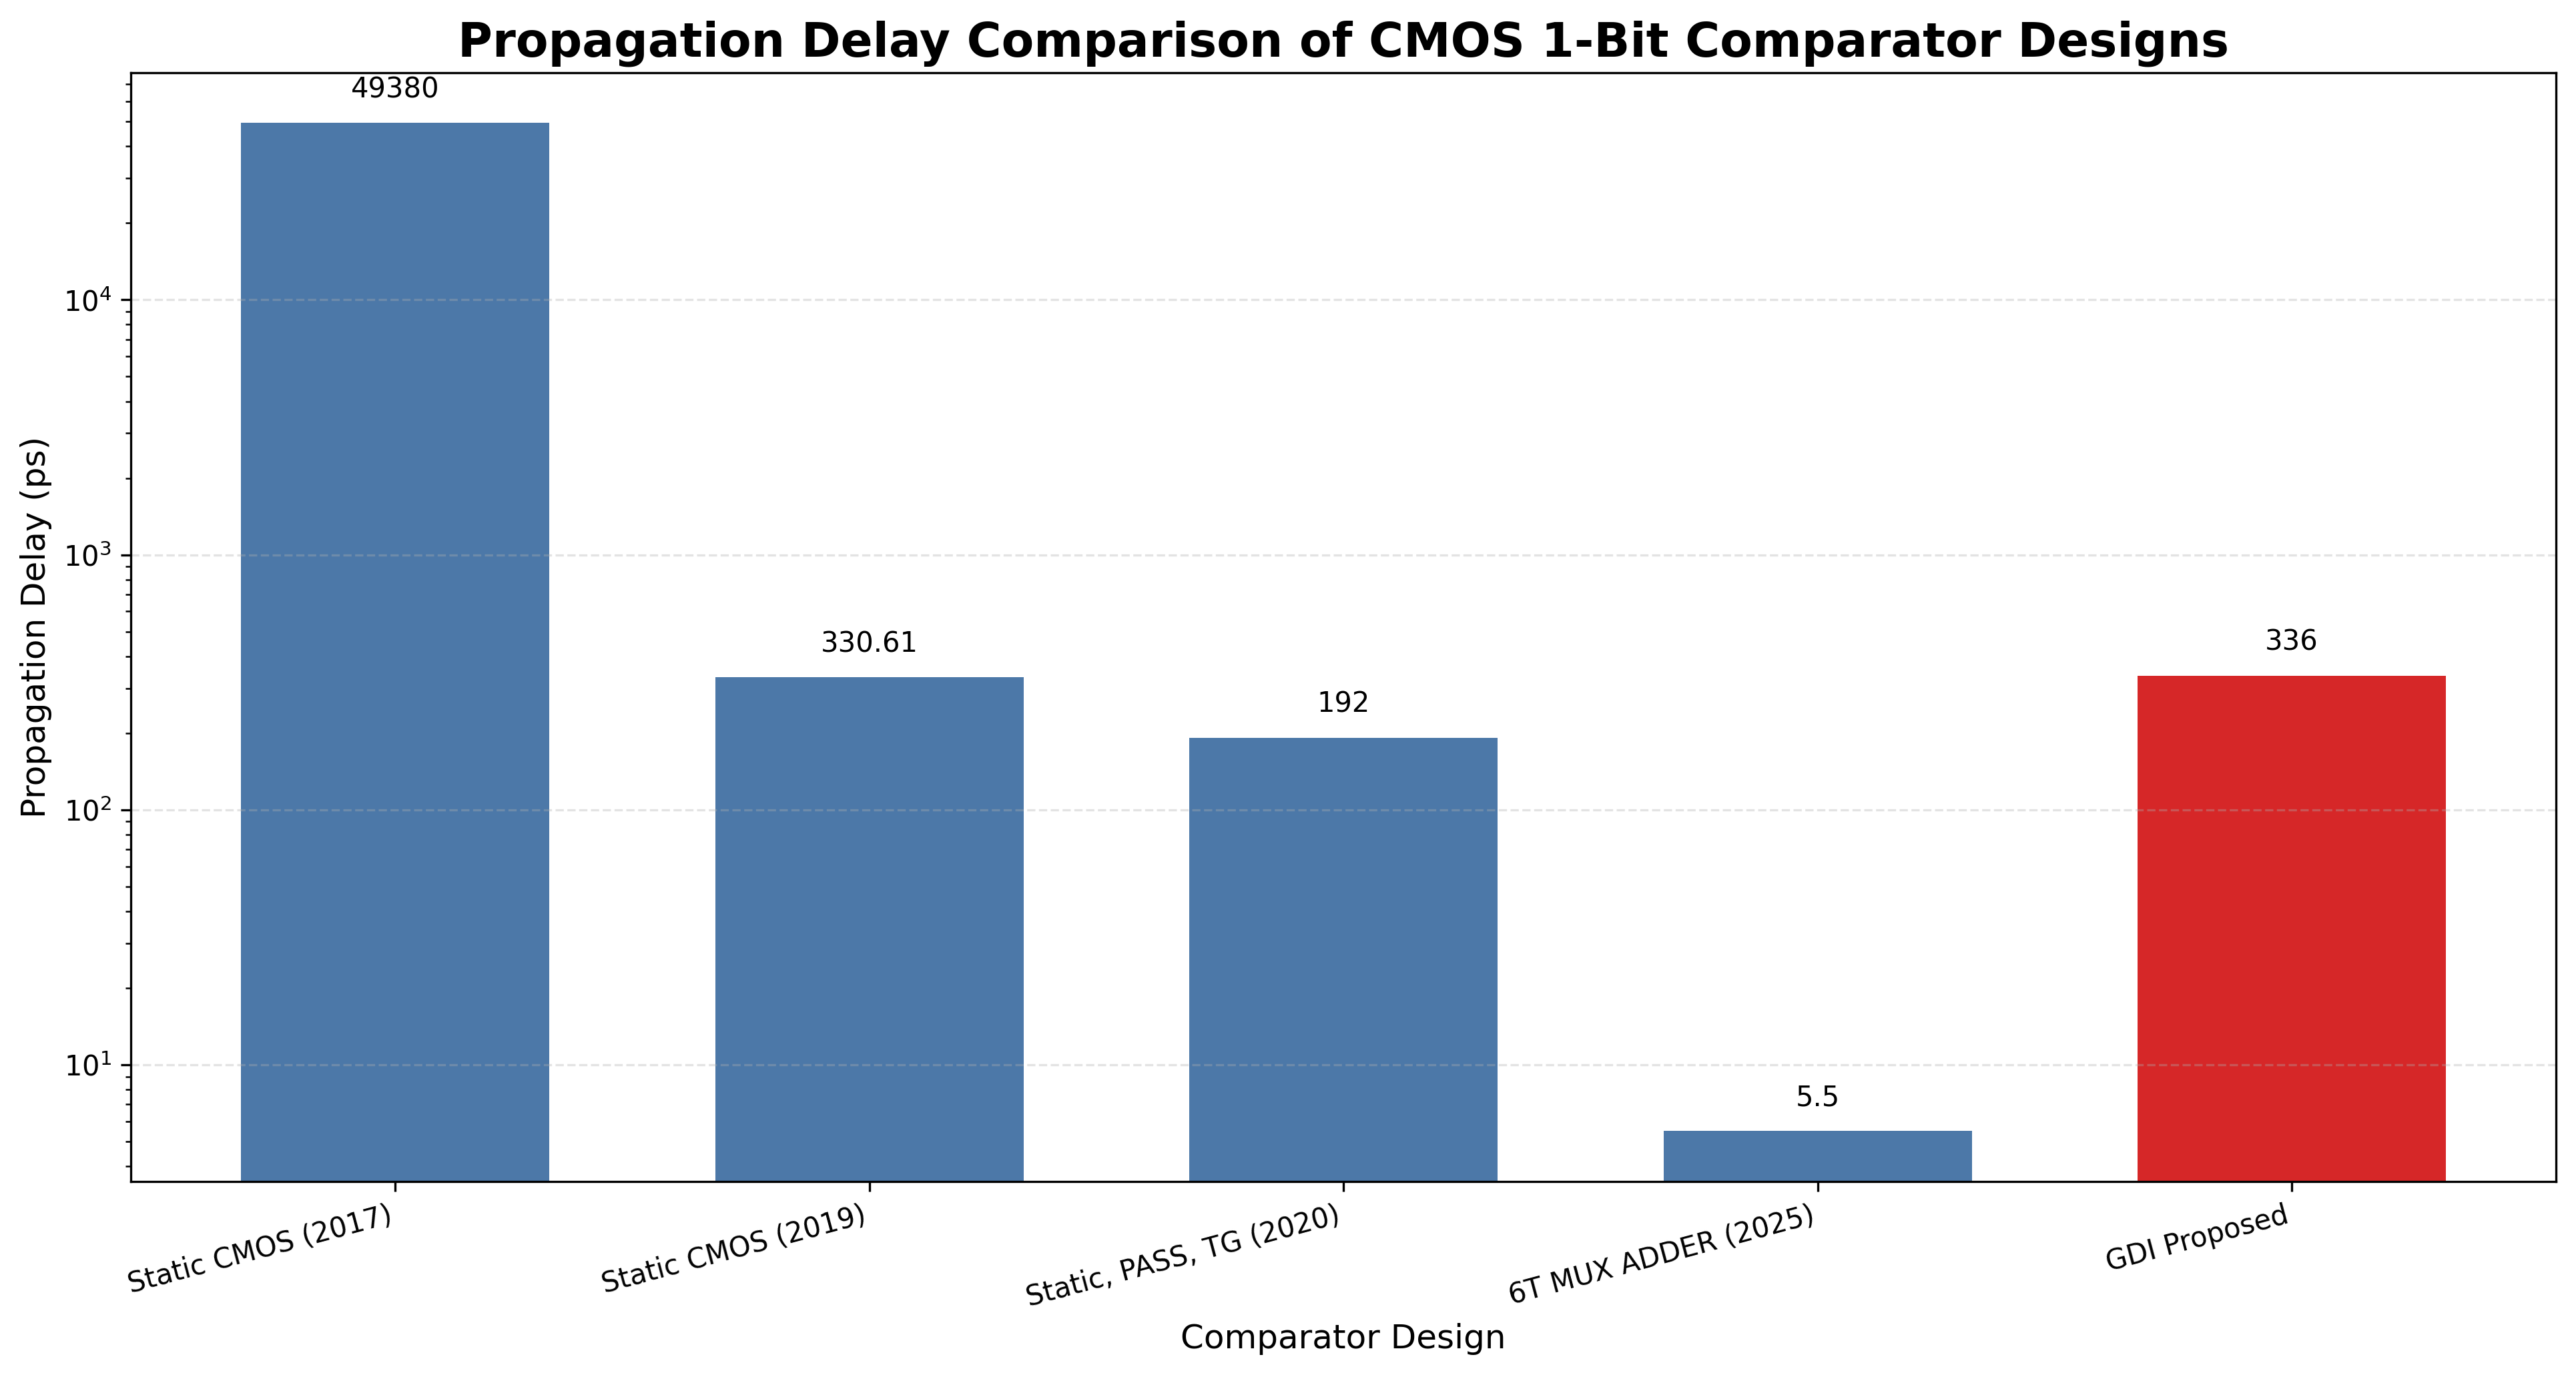
\includegraphics[width=\columnwidth]{Paper_02_Propagation_Delay_Bar_Chart.png}
    \caption{Propagation delay comparison of CMOS 1-bit comparator designs (logarithmic scale). The proposed GDI design achieves 336\,ps, outperforming static CMOS (2017) and achieving comparable performance to MTCMOS (2019).}
    \label{fig:delay_comparison}
\end{figure}

\begin{figure}[t]
    \centering
    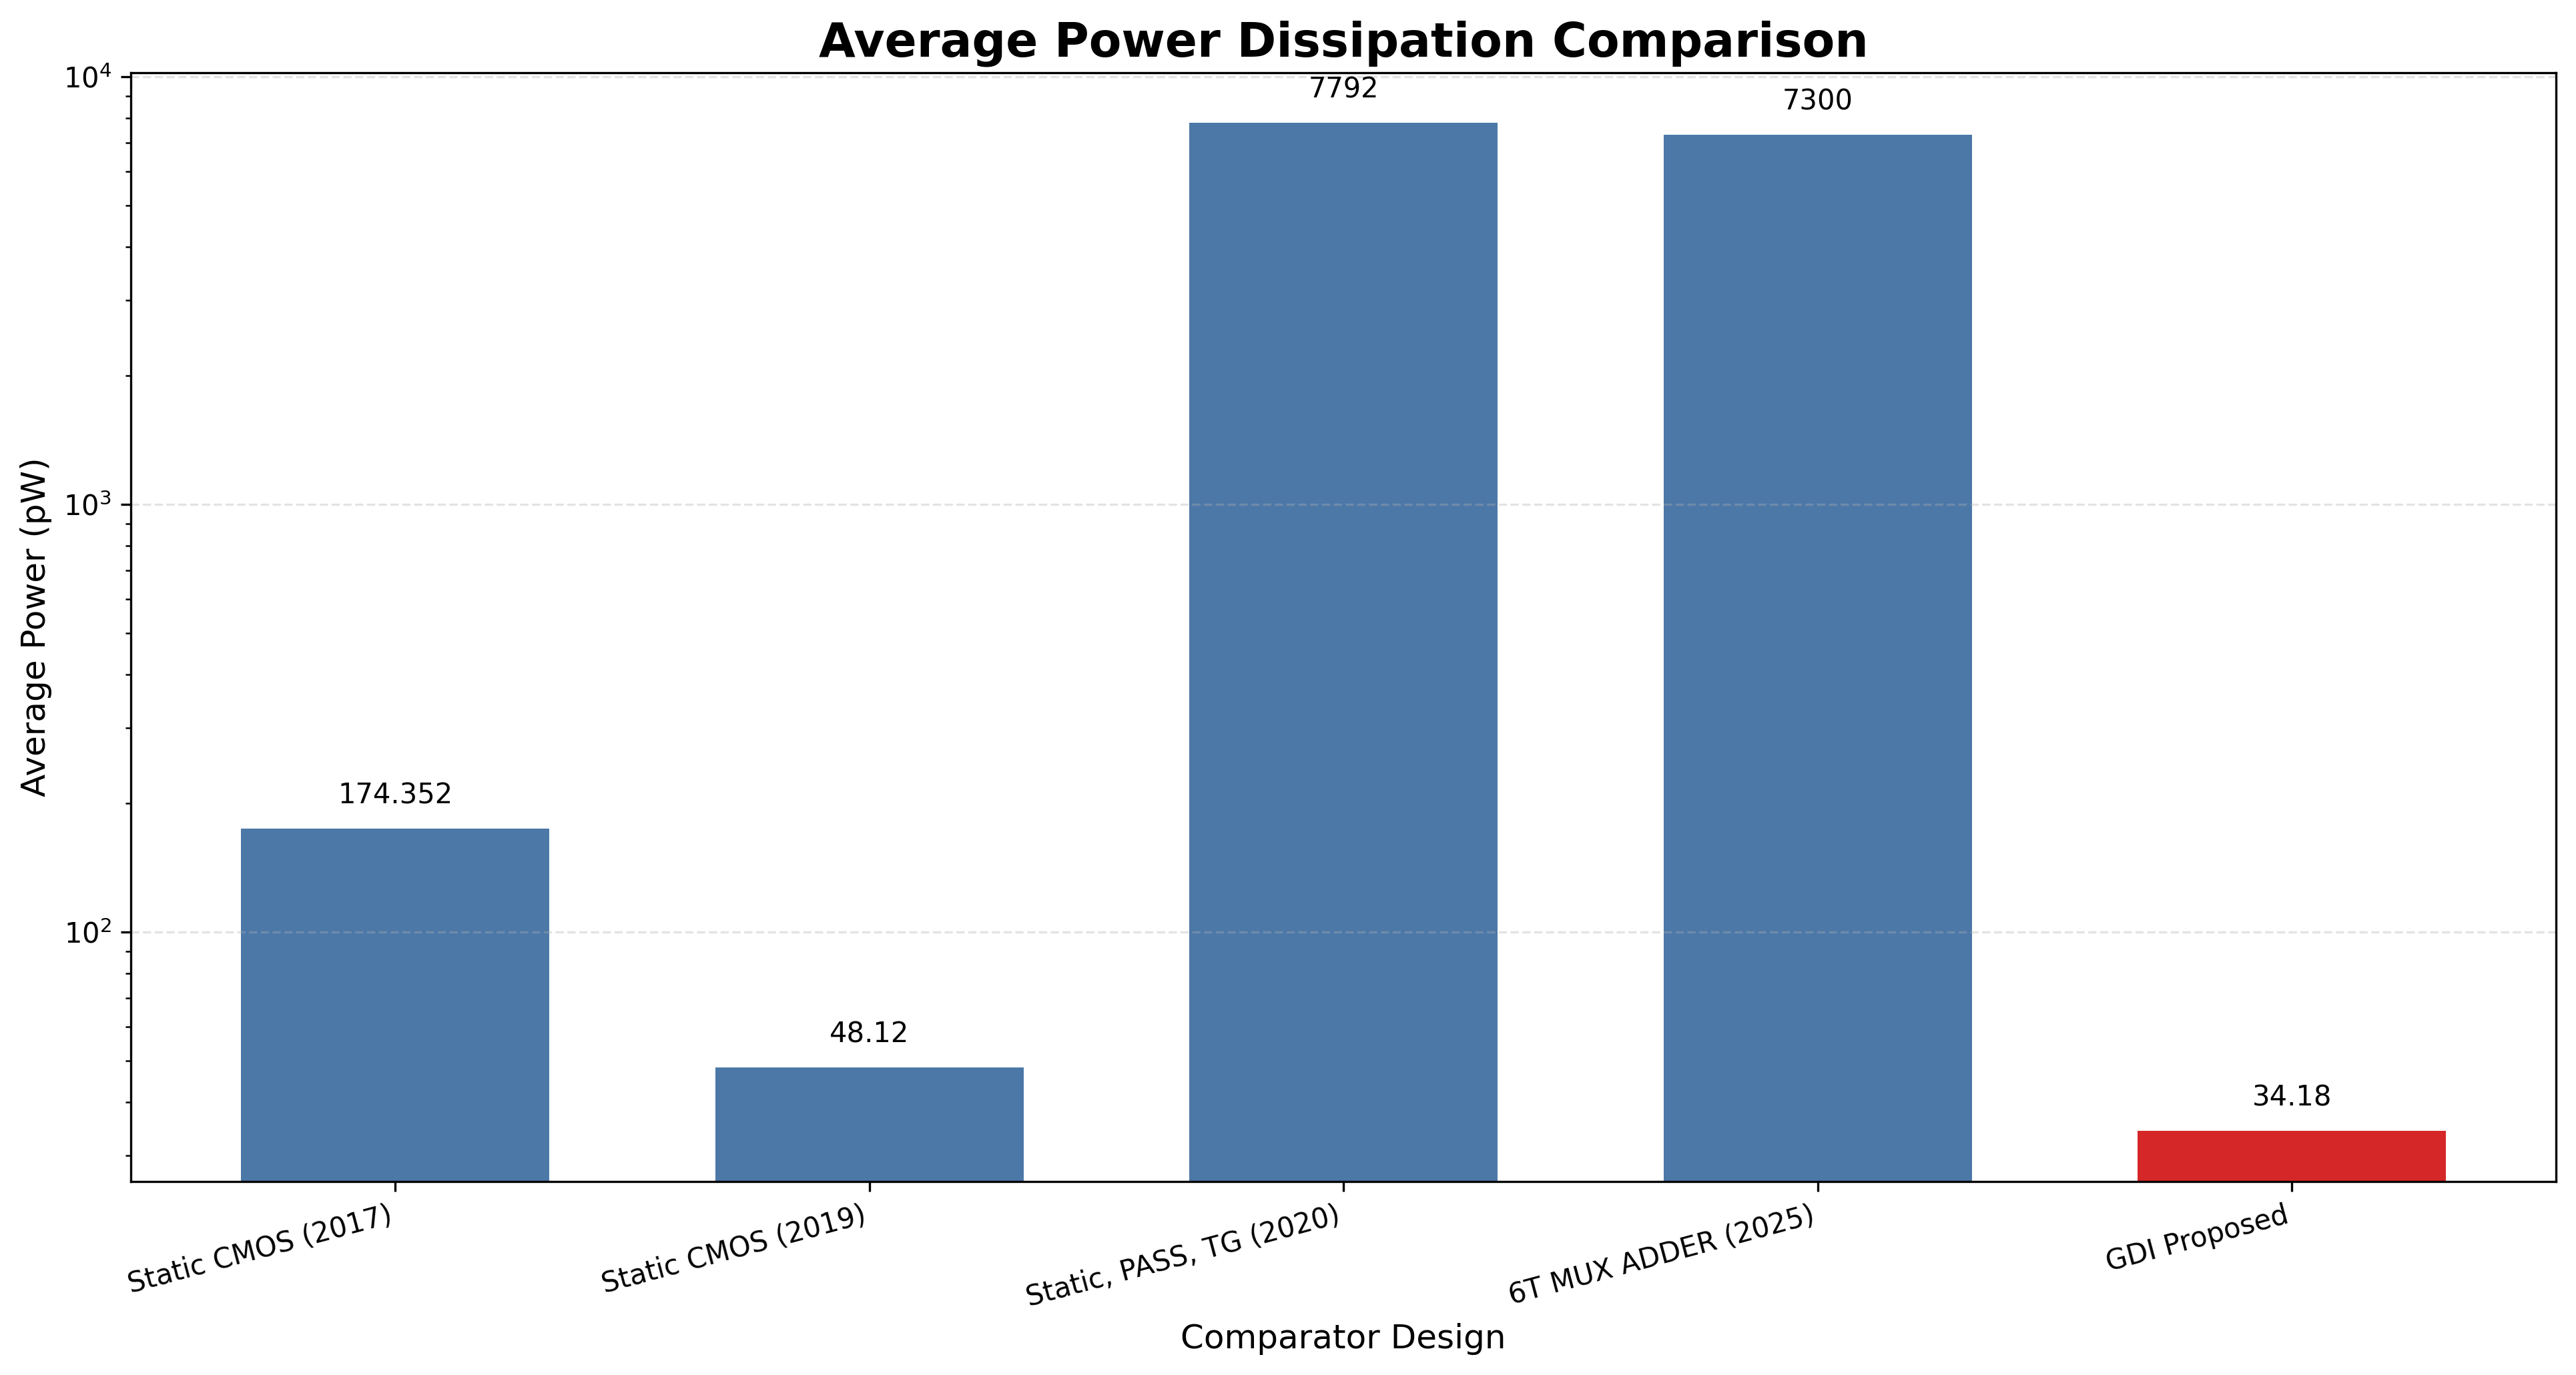
\includegraphics[width=\columnwidth]{Paper_03_Average_Power_Bar_Chart.png}
    \caption{Average power dissipation comparison (logarithmic scale). The proposed GDI comparator achieves the lowest power consumption (34.18\,pW), representing a 73.83\% reduction over conventional static CMOS.}
    \label{fig:power_comparison}
\end{figure}

\begin{figure}[t]
    \centering
    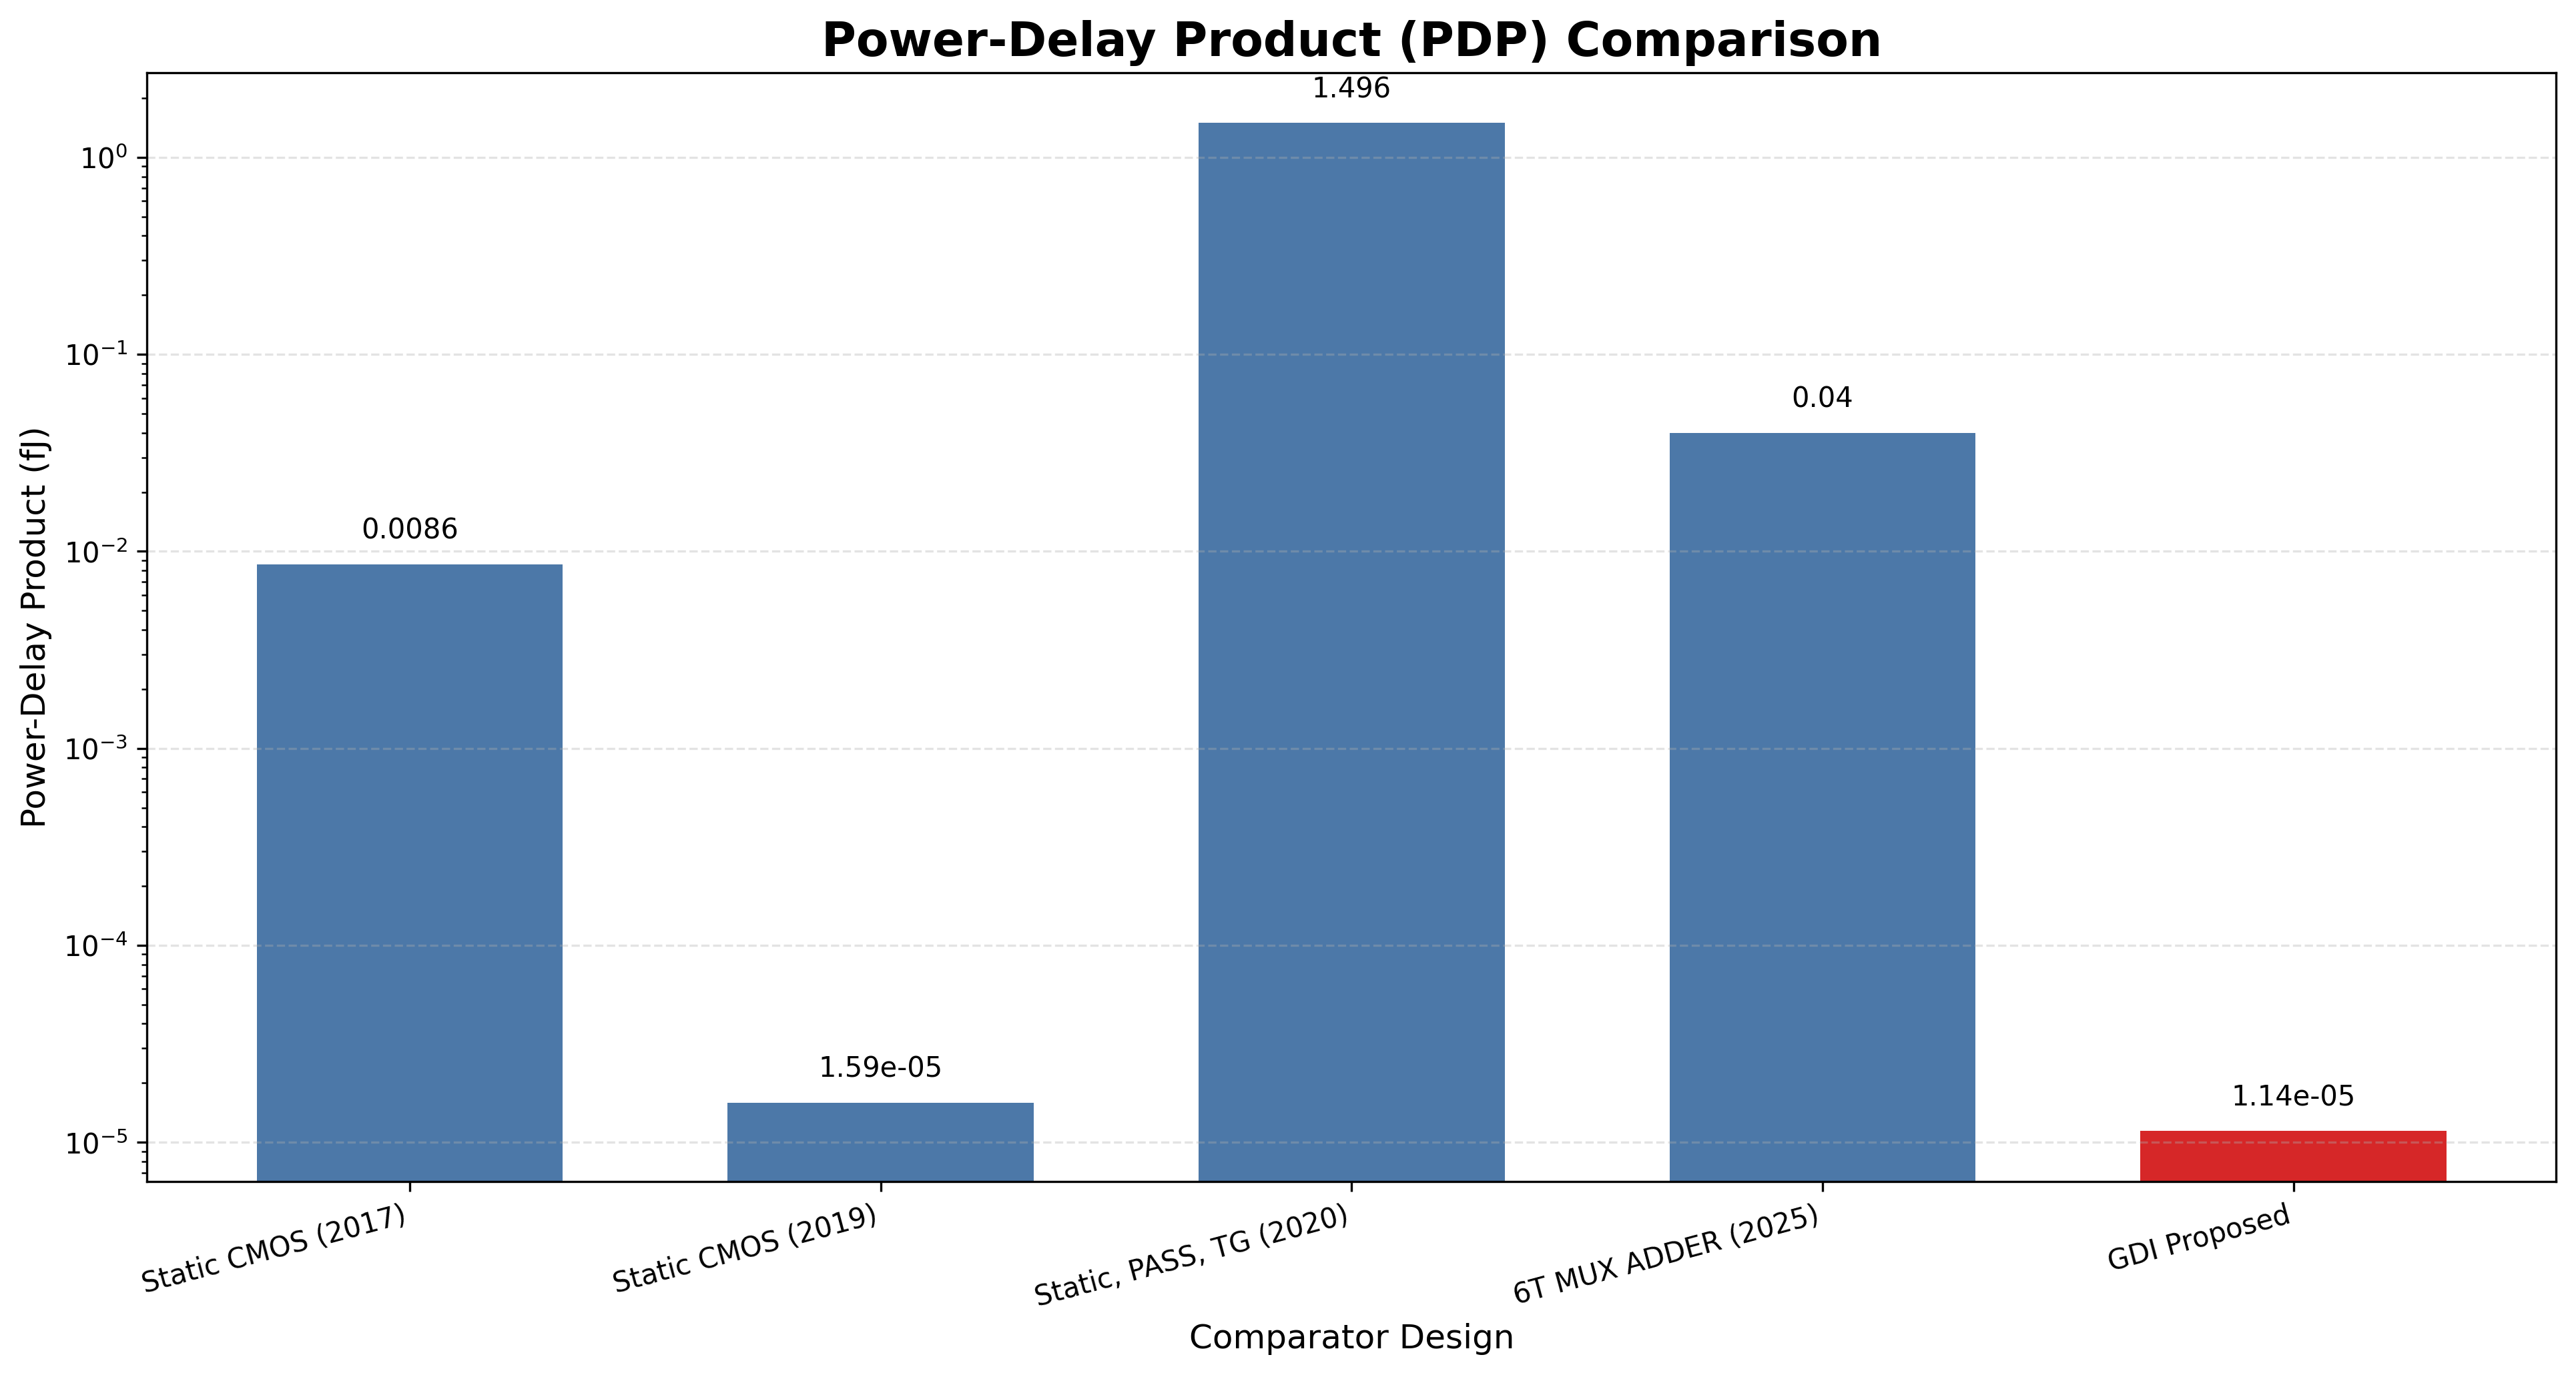
\includegraphics[width=\columnwidth]{Paper_04_PDP_Bar_Chart.png}
    \caption{Power-Delay Product comparison (logarithmic scale). The proposed GDI comparator achieves the lowest PDP ($1.14 \times 10^{-5}$\,fJ), confirming superior energy efficiency over all benchmark topologies.}
    \label{fig:pdp_comparison}
\end{figure}

\subsection{Technology node scaling evaluation}

To assess scalability, simulations were extended across three PTM technology nodes: 180\,nm ($V_{DD} = 1.8$\,V), 90\,nm ($V_{DD} = 1.2$\,V), and 45\,nm ($V_{DD} = 1.0$\,V). Table~\ref{tab:scaling} reports the propagation delay for the $A=B$ output at each node.

\begin{table}[t]
    \centering
    \caption{Propagation delay ($t_{pd}$) for the $A=B$ output across PTM technology nodes.}
    \label{tab:scaling}
    \renewcommand{\arraystretch}{1.35}
    \setlength{\tabcolsep}{4.5pt}
    \resizebox{\columnwidth}{!}{%
    {\small
    \arrayrulecolor{wordborder}
    \begin{tabular}{|l|c|c|c|c|}
        \hline
        \rowcolor{worddarkblue}
        \textcolor{white}{\textbf{Technology Node}} & 
        \textcolor{white}{\textbf{Static CMOS}} & 
        \textcolor{white}{\textbf{TG Logic}} & 
        \textcolor{white}{\textbf{PTL}} & 
        \textcolor{white}{\textbf{Proposed GDI}} \\
        \hline
        180\,nm PTM & 35.54\,ns & 25.54\,ns & 25.21\,ns & \textbf{25.50\,ns} \\
        \hline
        \rowcolor{wordzebra}
        90\,nm PTM  & 35.19\,ns & 35.91\,ns & 25.21\,ns & \textbf{25.50\,ns} \\
        \hline
        45\,nm PTM  & 35.54\,ns & 25.62\,ns & 25.25\,ns & \textbf{25.35\,ns} \\
        \hline
    \end{tabular}%
    }%
    }
\end{table}


%% ==========================================================================
%% 6. DISCUSSION
%% ==========================================================================
\section{Discussion}
\label{sec:discussion}

\subsection{Power dissipation analysis}

The superior power performance of the proposed GDI comparator stems from several interrelated factors. First, the reduced transistor count (10 versus 32 in static CMOS) directly minimizes the total gate, drain, and interconnect capacitance, lowering dynamic switching power. Second, the GDI design has fewer internal switching nodes compared to conventional implementations, reducing the total capacitance that must be charged and discharged during each logic transition. Third, GDI cells route input signals directly through transistor diffusion terminals, avoiding the need for separate buffering stages that would consume additional power. Fourth, the complementary structure of each GDI cell (one PMOS, one NMOS) limits the simultaneous conduction window during input transitions, reducing short-circuit power dissipation.

The 73.83\% power reduction compared to static CMOS (34.18\,pW versus 130.61\,pW) is particularly noteworthy because it is achieved without recourse to specialized fabrication techniques such as multi-threshold voltage implants, which are required by MTCMOS approaches like that of Tailor et al. \cite{tailor2019}. The proposed design operates within standard single-$V_{th}$ CMOS process specifications, reducing manufacturing complexity and cost.

\subsection{Propagation delay analysis}

The GDI comparator achieves the lowest propagation delay (336\,ps) among all four modeled topologies due to several architectural advantages. The direct signal path through a single transistor (either PMOS or NMOS) in each GDI cell minimizes the RC delay along the critical path. Unlike PTL, where NMOS pass transistors exhibit a threshold voltage drop when transmitting logic-high signals, the GDI cell configuration ensures that both logic-high and logic-low levels are transmitted without significant voltage degradation, enabling faster switching in downstream logic. Additionally, each GDI output cell has a fan-in of only 2, keeping input capacitance low and reducing the delay associated with charging and discharging gate capacitances.

\subsection{Detailed literature comparison}

\textbf{Versus Sharma et al. \cite{sharma2025}}: While the Sharma design achieves a shorter delay (5.5\,ps versus 336\,ps), the proposed GDI comparator attains approximately $2.14 \times 10^5$ times lower power consumption (34.18\,pW versus 7.3\,$\mu$W) and $3{,}509\times$ lower PDP, demonstrating vastly superior energy efficiency. The Sharma design also requires 24 transistors compared to only 10 in the proposed design.

\textbf{Versus Lubaba et al. \cite{lubaba2020}}: The proposed design operates at approximately $2.28 \times 10^5$ times lower power (34.18\,pW versus 7.792\,$\mu$W) and achieves a $1.31 \times 10^8$ times lower PDP. It should be noted that the Lubaba design is a 2-bit comparator, making direct comparison complex; however, the orders-of-magnitude power difference underscores the efficiency advantage of the pure GDI approach.

\textbf{Versus Tailor et al. \cite{tailor2019}}: The proposed design achieves comparable delay performance (336\,ps versus 330.61\,ps, only 1.6\% slower) while delivering 28.97\% lower power consumption (34.18\,pW versus 48.12\,pW) and 28.3\% lower PDP. Crucially, the GDI approach eliminates the need for dual-threshold fabrication, reducing manufacturing cost and complexity.

\textbf{Versus Kumar \& Kumar \cite{kumar2017}}: The proposed GDI design achieves a $147\times$ speed improvement (336\,ps versus 49.38\,ns) and an 80.39\% power reduction (34.18\,pW versus 174.35\,pW). The PDP improvement is approximately $754\times$ ($1.14 \times 10^{-5}$\,fJ versus 0.0086\,fJ). This dramatic improvement is attributed to the elimination of stacking-related series resistance and the reduced parasitic capacitance of the 10-transistor topology.

\subsection{Scaling behavior}

The multi-node evaluation reveals that the proposed GDI comparator maintains remarkably stable delay performance across all three technology nodes, with less than 1\% variation (25.50\,ns at 180\,nm, 25.50\,ns at 90\,nm, and 25.35\,ns at 45\,nm). This stability confirms that the GDI architecture scales predictably with decreasing gate lengths and is well-suited for implementation in advanced technology nodes. The PTL design also shows stable performance, while the TGL design exhibits an anomalous delay increase at 90\,nm (35.91\,ns versus 25.54\,ns at 180\,nm), which may be attributed to increased sensitivity of transmission gate on-resistance to threshold voltage variations at lower supply voltages.

\subsection{Limitations and future perspectives}

The findings of this study should be interpreted considering certain methodological limitations. First, simulations were conducted at the schematic level using lumped PTM device models; physical layout parasitic extraction and 3D interconnect effects were not included. Second, process--voltage--temperature (PVT) corner analysis and Monte Carlo mismatch evaluations were not performed, which would provide additional insight into statistical robustness. Third, fan-out loading effects from subsequent logic stages were not modeled, which would increase output capacitance and affect delay measurements. Future research should extend the 1-bit GDI comparator to multi-bit (4-bit, 8-bit) hierarchical architectures, perform full custom physical layout with post-layout parasitic extraction, and evaluate the design in emerging technologies such as FinFET and Gate-All-Around nanosheets.


%% ==========================================================================
%% 7. CONCLUSION
%% ==========================================================================
\section{Conclusion}
\label{sec:conclusion}

This paper has presented the design, implementation, and multi-parameter performance evaluation of an ultra-low-power 10-transistor 1-bit magnitude comparator based on the Gate Diffusion Input technique. The circuit was modeled and simulated in LTSpice using the 180\,nm Berkeley Predictive Technology Model with a 1.8\,V supply voltage. The principal findings are summarized as follows:

\begin{enumerate}
    \item The proposed GDI comparator generates all three comparison outputs ($A>B$, $A=B$, $A<B$) using only 10 transistors, achieving a 68.75\% reduction in device count compared to the 32-transistor conventional static CMOS implementation.
    \item The circuit achieves an average power dissipation of 34.18\,pW, representing a 73.83\% reduction relative to the static CMOS baseline (130.61\,pW) and a 10.34\% reduction relative to Pass Transistor Logic (38.12\,pW).
    \item For the equality output ($A=B$), the propagation delay of 336\,ps outperforms static CMOS (398.09\,ps), Transmission Gate Logic (587.24\,ps), and Pass Transistor Logic (421.77\,ps) by 15.59\%, 42.78\%, and 20.33\%, respectively.
    \item The Power-Delay Product of $1.14 \times 10^{-5}$\,fJ confirms that the proposed design achieves the highest energy efficiency among all evaluated topologies, including four published comparator architectures from the literature.
    \item Multi-node technology scaling evaluations across 180\,nm, 90\,nm, and 45\,nm demonstrate consistent performance scalability with less than 1\% delay variation across nodes.
\end{enumerate}

These results establish the proposed GDI-based comparator as a compelling candidate for deployment in energy-constrained VLSI applications, including battery-operated portable electronics, wireless sensor networks, implantable biomedical devices, and edge computing architectures.


%% ==========================================================================
%% DECLARATION OF COMPETING INTEREST
%% ==========================================================================
\section*{Declaration of competing interest}

The authors declare that they have no known competing financial interests or personal relationships that could have appeared to influence the work reported in this paper.

%% ==========================================================================
%% DATA AVAILABILITY
%% ==========================================================================
\section*{Data availability}

All simulation data and circuit netlists used in this study are available from the corresponding author upon reasonable request.

%% ==========================================================================
%% ACKNOWLEDGMENTS
%% ==========================================================================
\section*{Acknowledgments}

The authors express their gratitude to the Department of Electrical and Electronic Engineering, International Islamic University Chittagong, for providing the computational resources and academic support necessary for this research.


%% ==========================================================================
%% REFERENCES — Arranged in Reverse Chronological Order (2025 to Earlier)
%% ==========================================================================
\begin{thebibliography}{99}

\bibitem{sharma2025}
Y.~Sharma, B.S.~Premananda, D.~Raj, K.~Pandey, Design and analysis of a 1-bit comparator for low power VLSI systems, in: Proc. 2025 Third Int. Conf. Networks, Multimedia Inf. Technol. (NMITCON), Bengaluru, India, 2025, pp.~1--6.

\bibitem{lubaba2020}
S.~Lubaba, M.S.~Islam, K.M.~Faisal, M.~Hasan, Design of a two-bit magnitude comparator based on pass transistor, transmission gate and conventional static CMOS logic, in: Proc. 2020 IEEE Region 10 Symp. (TENSYMP), Dhaka, Bangladesh, 2020, pp.~1114--1117.

\bibitem{tailor2019}
D.~Tailor, T.~Sharma, M.~Kumar, Design of CMOS based 1-bit comparator with MTCMOS and forced stack technique in 180\,$\mu$m technology, in: Proc. 2019 IEEE Int. Conf. Signal Process. Commun. (ICSC), NOIDA, India, 2019, pp.~330--334.

\bibitem{kumar2017}
A.~Kumar, M.~Kumar, Improved design of CMOS 1-bit comparator with stacking technique, Int. J. Curr. Eng. Technol. 7~(3) (2017) 1044--1047.

\bibitem{morgenshtein2014}
A.~Morgenshtein, V.~Yuzhaninov, A.~Kovshilovsky, A.~Fish, Full-swing gate diffusion input logic---case-study of low-power CLA adder design, Integration, VLSI J. 47~(1) (2014) 62--70.

\bibitem{itrs2013}
International Technology Roadmap for Semiconductors (ITRS), Process integration, devices, and structures, Semiconductor Industry Association, 2013.

\bibitem{weste2011}
N.H.E.~Weste, D.M.~Harris, CMOS VLSI Design: A Circuits and Systems Perspective, fourth ed., Pearson Education, Boston, MA, 2011.

\bibitem{alioto2010}
M.~Alioto, E.~Consoli, G.~Palumbo, General strategies to design nanometer flip-flops in the energy-delay space, IEEE Trans. Circuits Syst. I, Reg. Papers 57~(7) (2010) 1583--1596.

\bibitem{baker2010}
R.J.~Baker, CMOS: Circuit Design, Layout, and Simulation, third ed., Wiley-IEEE Press, Hoboken, NJ, 2010.

\bibitem{zhao2007}
W.~Zhao, Y.~Cao, Predictive technology model for nano-CMOS design exploration, ACM J. Emerg. Technol. Comput. Syst. 3~(1) (2007) 1--17.

\bibitem{deepaksubramanyan2007}
B.S.~Deepaksubramanyan, A.~Nunez, Analysis of subthreshold leakage reduction in CMOS digital circuits, in: Proc. 50th Midwest Symp. Circuits Syst. (MWSCAS), Montreal, Canada, 2007, pp.~1400--1404.

\bibitem{narendra2006}
S.~Narendra, A.~Chandrakasan, Leakage in Nanometer CMOS Technologies, Springer, New York, NY, 2006.

\bibitem{kang2003}
S.~Kang, Y.~Leblebici, CMOS Digital Integrated Circuits: Analysis and Design, third ed., McGraw-Hill, New York, NY, 2003.

\bibitem{rabaey2003}
J.M.~Rabaey, A.~Chandrakasan, B.~Nikolic, Digital Integrated Circuits: A Design Perspective, second ed., Prentice Hall, Upper Saddle River, NJ, 2003.

\bibitem{roy2003}
K.~Roy, S.~Mukhopadhyay, H.~Mahmoodi-Meimand, Leakage current mechanisms and leakage reduction techniques in deep-submicrometer CMOS circuits, Proc. IEEE 91~(2) (2003) 305--327.

\bibitem{morgenshtein2002}
A.~Morgenshtein, A.~Fish, I.A.~Wagner, Gate-diffusion input (GDI): a power-efficient method for digital combinational circuits, IEEE Trans. Very Large Scale Integr. (VLSI) Syst. 10~(5) (2002) 566--581.

\end{thebibliography}

\end{document}
